\clearpage\section{Results}

% {This should include your data analysis and findings}

% \begin{figure}[H]
% \label{fig:prototype1}
% \centering
% 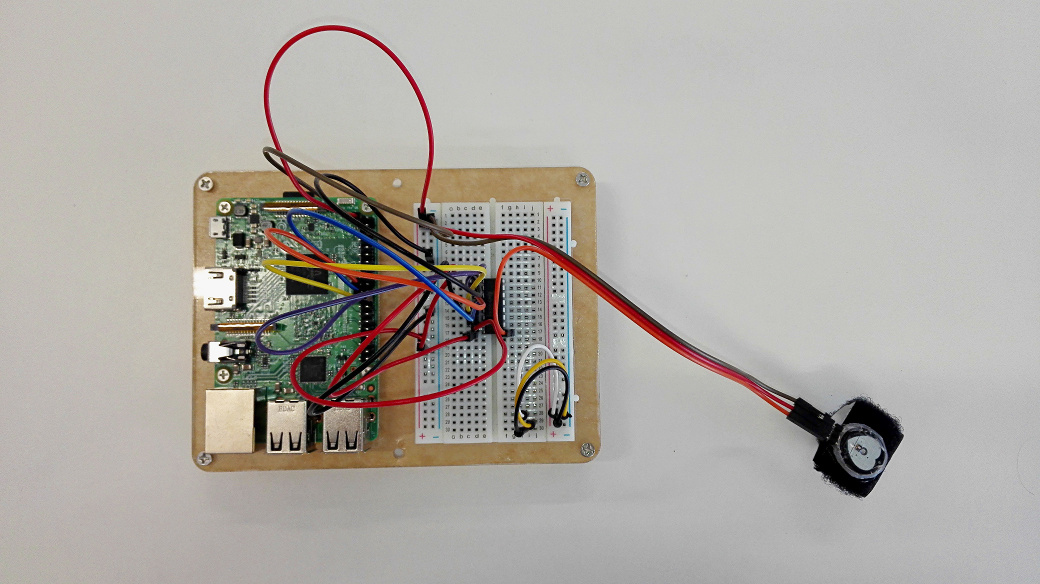
\includegraphics[width=10cm]{img/Chapter4/prototype1_edited.jpg}
% \caption[Prototype setup]{\footnotesize{Prototype setup.}}
% \end{figure}

% \begin{table}[H]
% \centering
% \caption[This is the caption]{ \footnotesize This is the other caption. Since the trial size of the experiments showed is one second, the number of \textit{Target} and \textit{Impostor} data corresponds to number of trials or seconds}
% \label{tab:data_partition}
% \footnotesize{
% \begin{tabular}{@{}llcccc@{}}
% \toprule
% \textbf{Dataset}         & \multicolumn{1}{c}{\textbf{Label}} & \textbf{Train} & \textbf{Validation} & \textbf{Develop} & \textbf{Test} \\ \midrule
% \midrule
% \multirow{3}{*}{First} & Target   & $135$ & $45$  & $30$  & $30$  \\
%                          & Impostor & $5,220$    & $1,740$ & $1,890$   & $2,880$    \\
% \cmidrule(lr){3-5} \cmidrule(l){6-6}
%                          & \#Subjects          & \multicolumn{3}{c}{$31$} & $12$ \\
% \midrule
% \multirow{3}{*}{Second}  & Target   & $144$ & $80$  & $48$  & $48$  \\
%                          & Impostor & $2,014$    & $1,119$    & $1,343$    & $1,545$ \\
% \cmidrule(lr){3-5} \cmidrule(l){6-6}
%                          & \#Subjects   & \multicolumn{3}{c}{$15$} & $5$ \\ 
% \bottomrule
% \end{tabular}
% }
% \end{table}

% \begin{algorithm}
\caption{Temperature-Distributed algorithm}\label{alg:tempdistrib}
\begin{algorithmic}[1]
\Procedure{Temp-Spread}{$GN_i, HN_j, temperatures$}\Comment{Lowest temperature priority}
\State $temperature\_list\gets short(temperatures)$
\State $max_temperature\gets max(temperature_list)$
\State $ThresHold\gets 0.5$
\State $temperature\_impact \gets 0.2$
\For{$GN_i$ in $i=1,8$}\Comment{Iterate every hardware node on the given GN}
\State $it\_temperature \gets temperature\_list(GN_i)$
\State $temp\_weight \gets \frac{max\_temperature-it\_temperature}{max\_temperature}*temperature\_impact$
\State $\omega(Master-GN_i) \gets ThresHold*temp\_weight$
\For{$HN_j$ in $j=1,n$}
\If{$available\_accel_{i,j} > busy\_accel_{i,j}$}
    \State $policy_\omega = \frac{Available HW}{Total HW}*ThresHold$
    \State $\omega(GN_i-HN_{i,j}) \gets ThresHold+policy_\omega$
\Else
    \State $\omega(GN_i - HN_{i,j}) \gets 1$
\EndIf

\EndFor
\EndFor
\State $node \gets find\_djistra\_shortest\_path(Master\_Node, aux\_node)$
\State \textbf{$return node$} $b$\Comment{The gcd is b}
\EndProcedure
\end{algorithmic}
\end{algorithm}

\subsection{Optimization of the code}

The first bottleneck found in the process of computing the histogram was the construction of the matrix $M$ itself. In the first iterations of the code we weren't considering the possibility of parallelizing, or even vectorizing the operations. When speaking of \textit{vectorizing} we refer to the use of numpy arrays and operations, which are optimized for numerical operations.

The initial implementation of the $M$ matrix calculation consisted on computing the matrix elements in a serial way, applying the hankel function to each element of the matrix. The approximate time of computing the whole matrix of dimension $N\times N \approx 700\times 700$ was around 20 seconds. Then, exploiting the fact that the matrix is symmetric, the time was reduced to around 10 seconds.

After this, an arcaic parallelisation scheme was proposed: the matrix was divided in four triangular blocks [make figure], and each block was computed in a different process. This computation was done initializing 4 different jobs with the multiprocessing library, and then joining the results. With this we achieved a time of 2.5 seconds for the whole matrix. Even though, the time was reduced by a factor of 8, it was still the bottleneck of the computation.

Finally, thanks to some training done externally, and by rethinking the way in which the matrix is constructed, the construction stopped being the bottleneck. With the help of the fact that numpy and scipy functions are optimized to work with array-like data, the construction was thought as follows:

\begin{enumerate}
    \item From the list of scatterers (array of dimension $(N,2)$ consisting on 2D vectors representing the coordinates of each scatterer) an upper diagonal matrix (without diagonal) is constructed, consisting on the value of the distance of dispersor $i$ with dispersor $j$. That is:
    \begin{equation}
        \mathcal{D}_{ij}=\begin{cases}
            |r_i-r_j|& i<j\\
            0&else
        \end{cases}
    \end{equation}
    This matrix is computed using numba's njit decorator [ANNEX?]
    \item This matrix is then multiplied by the momentum of the free particle. This basically is an upper triangular matrix that contains the argument of the hankel function.
    \item Then, the hankel function is applied once to the whole matrix, reducing the for loops needed.
    \item The transposed matrix is added to the upper triangular matrix.
    \item Finally, the diagonal is added.
\end{enumerate}
